% ==============================================================================
% BỘ ĐỀ THAM KHẢO TUYỂN SINH 10 NĂM HỌC 2026-2027 SỞ GD&ĐT TP.HCM
% ĐỢT 8: CỤM 6 - ĐỀ 1 & CỤM 6 - ĐỀ 2 (14 CÂU TỰ LUẬN)
% ==============================================================================

% ==============================================================================
% CỤM 6 - ĐỀ THAM KHẢO 1
% ==============================================================================

\begin{bt}%[9D6H18-2]
% nguon: Đề tham khảo Tuyển sinh 10 năm học 2026-2027 Sở GD&ĐT TP.HCM - Cụm 6 Đề 1, Bài 1
	Cho parabol $(P)\colon y = -\dfrac{1}{3}x^2$.
	\begin{enumerate}[a)]
		\item Vẽ đồ thị $(P)$.
		\item Tìm các điểm $N$ thuộc $(P)$ (khác gốc tọa độ $O$) sao cho tung độ gấp $3$ lần hoành độ.
	\end{enumerate}
	\loigiai{
		\begin{enumerate}[a)]
			\item Bảng giá trị tương ứng giữa $x$ và $y$ của parabol $(P)\colon y = -\dfrac{1}{3}x^2$:
			\begin{center}
				\begin{tabular}{|c|c|c|c|c|c|}
					\hline
					$x$ & $-6$ & $-3$ & $0$ & $3$ & $6$ \\
					\hline
					$y = -\dfrac{1}{3}x^2$ & $-12$ & $-3$ & $0$ & $-3$ & $-12$ \\
					\hline
				\end{tabular}
			\end{center}
			Đồ thị $(P)$ là một parabol đi qua gốc tọa độ $O(0;0)$ và nhận trục tung $Oy$ làm trục đối xứng.
			\begin{center}
				\begin{tikzpicture}[>=stealth, scale=0.6]
					\draw[->] (-7,0) -- (7,0) node[below] {$x$};
					\draw[->] (0,-13) -- (0,2) node[left] {$y$};
					\fill (0,0) circle (1.5pt) node[above right] {$O$};
					\draw[smooth, samples=100, domain=-6.2:6.2, thick, color=blue] plot(\x, {-1/3*(\x)^2});
					\draw[dashed] (-3,0) node[above] {$-3$} -- (-3,-3) -- (0,-3) node[right] {$-3$} -- (3,-3) -- (3,0) node[above] {$3$};
					\draw[dashed] (-6,0) node[above] {$-6$} -- (-6,-12) -- (0,-12) node[right] {$-12$} -- (6,-12) -- (6,0) node[above] {$6$};
					\fill (-3,-3) circle (1.5pt) (3,-3) circle (1.5pt) (-6,-12) circle (1.5pt) (6,-12) circle (1.5pt);
				\end{tikzpicture}
			\end{center}
			\item Gọi tọa độ điểm $N(x_N; y_N) \in (P)$.
			
			Vì tung độ gấp $3$ lần hoành độ nên $y_N = 3x_N$.
			
			Mặt khác, $N \in (P)$ nên $y_N = -\dfrac{1}{3}x_N^2$. Do đó:
			$$-\dfrac{1}{3}x_N^2 = 3x_N \iff x_N^2 + 9x_N = 0 \iff x_N(x_N + 9) = 0 \iff \left[\begin{aligned} &x_N = 0 \\ &x_N = -9. \end{aligned}\right.$$
			Vì $N \neq O$ nên $x_N \neq 0$, suy ra $x_N = -9$.
			
			Với $x_N = -9 \implies y_N = 3 \cdot (-9) = -27$.
			
			Vậy tọa độ điểm cần tìm là $N(-9; -27)$.
		\end{enumerate}
	}
\end{bt}

\begin{bt}%[9D6H20-2]
% nguon: Đề tham khảo Tuyển sinh 10 năm học 2026-2027 Sở GD&ĐT TP.HCM - Cụm 6 Đề 1, Bài 2
	Cho phương trình $2x^2 - 6x + 1 = 0$ có hai nghiệm phân biệt $x_1, x_2$. Không giải phương trình, hãy tính giá trị của biểu thức:
	$$A = 3x_1^2 x_2 + 3x_1 x_2^2 - x_1 - x_2.$$
	\loigiai{
		Phương trình $2x^2 - 6x + 1 = 0$ có:
		$$\Delta' = (-3)^2 - 2 \cdot 1 = 7 > 0$$
		nên phương trình luôn có hai nghiệm phân biệt $x_1, x_2$.
		
		Theo định lí Viète, ta có:
		$$\begin{cases} x_1 + x_2 = \dfrac{6}{2} = 3 \\ x_1 x_2 = \dfrac{1}{2}. \end{cases}$$
		Ta biến đổi biểu thức $A$:
		$$A = 3x_1 x_2(x_1 + x_2) - (x_1 + x_2).$$
		Thay $x_1 + x_2 = 3$ và $x_1 x_2 = \dfrac{1}{2}$ vào $A$, ta được:
		$$A = 3 \cdot \dfrac{1}{2} \cdot 3 - 3 = \dfrac{9}{2} - 3 = \dfrac{3}{2}.$$
		Vậy $A = \dfrac{3}{2}$.
	}
\end{bt}

\begin{bt}%[9D8H26-3]
% nguon: Đề tham khảo Tuyển sinh 10 năm học 2026-2027 Sở GD&ĐT TP.HCM - Cụm 6 Đề 1, Bài 3
	Biểu đồ thống kê số học sinh nam và số học sinh nữ tham gia Hội khỏe Phù Đổng cấp Thành phố của một trường trung học cơ sở:
	\begin{center}
		\begin{tabular}{|l|c|c|c|c|}
			\hline
			\textbf{Khối} & Khối 6 & Khối 7 & Khối 8 & Khối 9 \\
			\hline
			\textbf{Số học sinh nam} & 6 & 9 & 8 & 8 \\
			\hline
			\textbf{Số học sinh nữ} & 8 & 7 & 9 & 7 \\
			\hline
		\end{tabular}
	\end{center}
	Chọn ngẫu nhiên một học sinh trong danh sách tham gia thi đấu.
	\begin{enumerate}[a)]
		\item Tính tổng số học sinh của trường tham gia Hội khỏe Phù Đổng cấp Thành phố.
		\item Tính xác suất của biến cố $A$: ``Học sinh được chọn là học sinh nam''.
		\item Tính xác suất của biến cố $B$: ``Học sinh được chọn là học sinh khối 9''.
	\end{enumerate}
	\loigiai{
		\begin{enumerate}[a)]
			\item Tổng số học sinh của trường tham gia Hội khỏe Phù Đổng là:
			$$(6 + 8) + (9 + 7) + (8 + 9) + (8 + 7) = 14 + 16 + 17 + 15 = 62\text{ (học sinh)}.$$
			\item Số học sinh nam tham gia là:
			$$6 + 9 + 8 + 8 = 31\text{ (học sinh)}.$$
			Xác suất của biến cố $A$ là:
			$$P(A) = \dfrac{31}{62} = \dfrac{1}{2} = 0{,}5.$$
			\item Số học sinh khối 9 tham gia là:
			$$8 + 7 = 15\text{ (học sinh)}.$$
			Xác suất của biến cố $B$ là:
			$$P(B) = \dfrac{15}{62}.$$
		\end{enumerate}
	}
\end{bt}

\begin{bt}%[9D6V21-3]
% nguon: Đề tham khảo Tuyển sinh 10 năm học 2026-2027 Sở GD&ĐT TP.HCM - Cụm 6 Đề 1, Bài 4
	Một sân bóng mini hình chữ nhật có kích thước $15\text{ m} \times 6\text{ m}$. Người ta muốn làm một lối đi bao gồm một lối đi dọc và một lối đi ngang có cùng bề rộng $x\text{ (m)}$ ($x > 0$), khi đó khu đất mới có kích thước là $(15 + x)\text{ m}$ và $(6 + x)\text{ m}$.
	\begin{enumerate}[a)]
		\item Hãy biểu diễn diện tích $S$ của lối đi theo $x$.
		\item Biết diện tích lối đi là $46\text{ m}^2$, hãy tính bề rộng $x$ của lối đi.
	\end{enumerate}
	\loigiai{
		\begin{enumerate}[a)]
			\item Diện tích sân bóng ban đầu là:
			$$15 \cdot 6 = 90\text{ (m}^2).$$
			Diện tích của toàn bộ khu đất bao gồm sân và lối đi là:
			$$(15 + x)(6 + x) = x^2 + 21x + 90\text{ (m}^2).$$
			Diện tích của phần lối đi là:
			$$S = (x^2 + 21x + 90) - 90 = x^2 + 21x\text{ (m}^2).$$
			\item Theo đề bài, diện tích lối đi là $46\text{ m}^2$ nên ta có phương trình:
			$$x^2 + 21x = 46 \iff x^2 + 21x - 46 = 0.$$
			Ta có $\Delta = 21^2 - 4 \cdot 1 \cdot (-46) = 441 + 184 = 625 = 25^2 > 0$.
			
			Phương trình có hai nghiệm phân biệt:
			$$x_1 = \dfrac{-21 + 25}{2} = 2\text{ (thỏa mãn } x > 0),\quad x_2 = \dfrac{-21 - 25}{2} = -23\text{ (loại)}.$$
			Vậy bề rộng của lối đi là $2\text{ m}$.
		\end{enumerate}
	}
\end{bt}

\begin{bt}%[9H0V31-3]
% nguon: Đề tham khảo Tuyển sinh 10 năm học 2026-2027 Sở GD&ĐT TP.HCM - Cụm 6 Đề 1, Bài 5
	Một người nông dân dùng đôi quang gánh để gánh hai thúng gạo giống hệt nhau. Mỗi thúng gạo gồm phần đáy là một nửa hình cầu có đường kính $40\text{ cm}$ và phần trên vun lên thành hình nón có chiều cao $15\text{ cm}$.
	\begin{enumerate}[a)]
		\item Tính thể tích gạo chứa đầy trong một chiếc thúng (kết quả làm tròn đến hàng đơn vị của $\text{cm}^3$). Cho biết công thức thể tích hình cầu $V = \dfrac{4}{3}\pi R^3$ và thể tích hình nón $V = \dfrac{1}{3}\pi R^2 h$.
		\item Người đó dùng một chiếc lon hình trụ có đường kính đáy $8\text{ cm}$ và chiều cao $10\text{ cm}$ để đong hết số gạo trong cả hai chiếc thúng. Mỗi lần đong, lượng gạo trong lon chỉ đạt $95\%$ thể tích lon. Hỏi cần đong ít nhất bao nhiêu lần để đong hết số gạo trong cả hai thúng?
	\end{enumerate}
	\loigiai{
		\begin{enumerate}[a)]
			\item Bán kính đáy của nửa hình cầu và hình nón là:
			$$R = \dfrac{40}{2} = 20\text{ (cm)}.$$
			Thể tích phần nửa hình cầu ở đáy thúng là:
			$$V_1 = \dfrac{1}{2} \cdot \left(\dfrac{4}{3}\pi R^3\right) = \dfrac{2}{3}\pi \cdot 20^3 = \dfrac{16000}{3}\pi\text{ (cm}^3).$$
			Thể tích phần hình nón vun lên là:
			$$V_2 = \dfrac{1}{3}\pi R^2 h = \dfrac{1}{3}\pi \cdot 20^2 \cdot 15 = 2000\pi = \dfrac{6000}{3}\pi\text{ (cm}^3).$$
			Thể tích gạo chứa trong một chiếc thúng là:
			$$V = V_1 + V_2 = \dfrac{16000}{3}\pi + \dfrac{6000}{3}\pi = \dfrac{22000}{3}\pi \approx 23038\text{ (cm}^3).$$
			\item Bán kính đáy của lon hình trụ là:
			$$r = \dfrac{8}{2} = 4\text{ (cm)}.$$
			Thể tích của lon hình trụ là:
			$$V_{\text{lon}} = \pi r^2 h_{\text{lon}} = \pi \cdot 4^2 \cdot 10 = 160\pi\text{ (cm}^3).$$
			Lượng gạo thực tế đong được trong mỗi lần là:
			$$V_{\text{đong}} = 95\% \cdot V_{\text{lon}} = 0{,}95 \cdot 160\pi = 152\pi\text{ (cm}^3).$$
			Tổng lượng gạo có trong cả hai thúng là:
			$$2V = 2 \cdot \dfrac{22000}{3}\pi = \dfrac{44000}{3}\pi\text{ (cm}^3).$$
			Số lần đong gạo cần thiết là:
			$$n = \dfrac{2V}{V_{\text{đong}}} = \dfrac{\dfrac{44000\pi}{3}}{152\pi} = \dfrac{44000}{3 \cdot 152} = \dfrac{44000}{456} \approx 96{,}49.$$
			Vì số lần đong phải là số nguyên nên người đó cần đong ít nhất $97$ lần để hết toàn bộ số gạo trong cả hai thúng.
		\end{enumerate}
	}
\end{bt}

\begin{bt}%[9D1H3-4]
% nguon: Đề tham khảo Tuyển sinh 10 năm học 2026-2027 Sở GD&ĐT TP.HCM - Cụm 6 Đề 1, Bài 6
	Lớp 9A có $45$ học sinh gồm $27$ học sinh nam và $18$ học sinh nữ tham gia hoạt động thiện nguyện làm thiệp và gấp hạc giấy tặng các em nhỏ vùng cao. Bạn An là một học sinh nam của lớp. Mỗi bạn nam khác bạn An đều làm được $3$ tấm thiệp. Các bạn nữ trong lớp, mỗi bạn gấp được $2$ con hạc hoặc $5$ con hạc giấy. Sau buổi hoạt động, số hạc giấy gấp được bằng tổng số tấm thiệp mà các bạn nam (khác bạn An) làm được. Hỏi có bao nhiêu bạn nữ gấp được $2$ con hạc và bao nhiêu bạn nữ gấp được $5$ con hạc giấy?
	\loigiai{
		Số bạn nam khác bạn An trong lớp là:
		$$27 - 1 = 26\text{ (học sinh)}.$$
		Tổng số tấm thiệp mà các bạn nam (khác An) làm được là:
		$$26 \cdot 3 = 78\text{ (tấm thiệp)}.$$
		Do đó tổng số hạc giấy mà $18$ bạn nữ gấp được là $78$ con hạc.
		
		Gọi $x$ là số bạn nữ gấp được $2$ con hạc giấy ($x \in \mathbb{N}^*$, $x < 18$).
		
		Gọi $y$ là số bạn nữ gấp được $5$ con hạc giấy ($y \in \mathbb{N}^*$, $y < 18$).
		
		Vì lớp có $18$ bạn nữ nên ta có phương trình:
		$$x + y = 18. \quad (1)$$
		Vì tổng số hạc giấy gấp được là $78$ nên ta có phương trình:
		$$2x + 5y = 78. \quad (2)$$
		Từ $(1)$ và $(2)$, ta có hệ phương trình:
		$$\begin{cases} x + y = 18 \\ 2x + 5y = 78 \end{cases} \iff \begin{cases} 2x + 2y = 36 \\ 2x + 5y = 78 \end{cases} \iff \begin{cases} 3y = 42 \\ x = 18 - y \end{cases} \iff \begin{cases} y = 14\text{ (nhận)} \\ x = 4\text{ (nhận)}. \end{cases}$$
		Vậy có $4$ bạn nữ gấp được $2$ con hạc và $14$ bạn nữ gấp được $5$ con hạc giấy.
	}
\end{bt}

\begin{bt}%[9H9C29-3]
% nguon: Đề tham khảo Tuyển sinh 10 năm học 2026-2027 Sở GD&ĐT TP.HCM - Cụm 6 Đề 1, Bài 7
	Cho đường tròn $(O; R)$ và đường thẳng $d$ không cắt đường tròn $(O)$. Kẻ $OH \perp d$ tại $H$. Lấy điểm $K$ tùy ý trên đường thẳng $d$ ($K$ không trùng với $H$). Từ $K$ kẻ hai tiếp tuyến $KA, KB$ với $(O)$ ($A, B$ là hai tiếp điểm). Dây $AB$ cắt đoạn thẳng $OH$ tại $I$.
	\begin{enumerate}[a)]
		\item Chứng minh bốn điểm $K, A, O, H$ cùng thuộc một đường tròn.
		\item Chứng minh $IA \cdot IB = IH \cdot IO$.
		\item Cho biết $OK = 2R$ và $OH = R\sqrt{3}$. Tính diện tích tam giác $KAB$ theo $R$.
	\end{enumerate}
	\loigiai{
		\begin{center}
			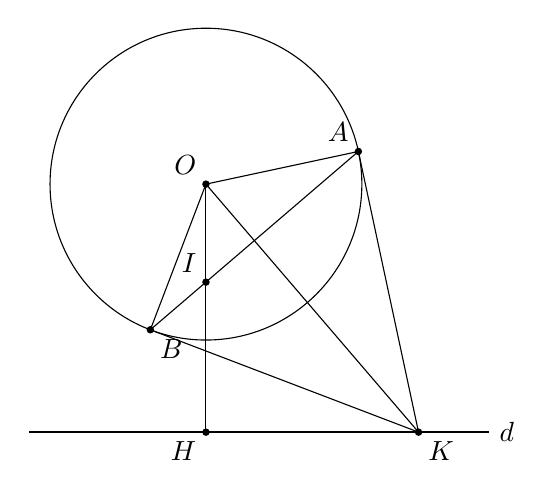
\begin{tikzpicture}[>=stealth, scale=0.9]
				\coordinate (O) at (0,0);
				\def\r{2.2}
				\draw (O) circle (\r);
				\coordinate (H) at (0,-3.5);
				\draw[thick] (-2.5,-3.5) -- (4,-3.5) node[right] {$d$};
				\coordinate (K) at (3,-3.5);
				\node at (O) [above left] {$O$};
				\node at (H) [below left] {$H$};
				\node at (K) [below right] {$K$};
				\pgfmathsetmacro{\distOK}{sqrt(3^2 + 3.5^2)}
				\pgfmathsetmacro{\angOK}{atan2(-3.5,3)}
				\pgfmathsetmacro{\alphaVal}{acos(\r/\distOK)}
				\coordinate (A) at ({\angOK + \alphaVal}:\r);
				\coordinate (B) at ({\angOK - \alphaVal}:\r);
				\draw (K) -- (A) node[above left] {$A$};
				\draw (K) -- (B) node[below right] {$B$};
				\draw (O) -- (A);
				\draw (O) -- (B);
				\draw (O) -- (K);
				\draw (O) -- (H);
				\draw (A) -- (B);
				\coordinate (I) at (intersection of A--B and O--H);
				\node at (I) [above left] {$I$};
				\fill (O) circle (1.5pt) (H) circle (1.5pt) (K) circle (1.5pt) (A) circle (1.5pt) (B) circle (1.5pt) (I) circle (1.5pt);
			\end{tikzpicture}
		\end{center}
		\begin{enumerate}[a)]
			\item Vì $KA$ là tiếp tuyến của $(O)$ nên $KA \perp OA \implies \widehat{KAO} = 90^\circ$.
			
			Vì $OH \perp d$ tại $H$ và $K \in d$ nên $\widehat{KHO} = 90^\circ$.
			
			Tứ giác $KAOH$ có $\widehat{KAO} = \widehat{KHO} = 90^\circ$, do đó hai đỉnh $A$ và $H$ cùng nhìn đoạn $KO$ dưới một góc vuông.
			
			Suy ra bốn điểm $K, A, O, H$ cùng thuộc đường tròn đường kính $KO$.
			\item Gọi $M$ là giao điểm của $OK$ và $AB$.
			
			Vì $KA, KB$ là hai tiếp tuyến cắt nhau nên $KA = KB$ và $OA = OB = R$.
			
			Do đó $OK$ là đường trung trực của đoạn thẳng $AB$, suy ra $OK \perp AB$ tại $M$.
			
			Xét $\Delta OMI$ và $\Delta OHK$ có:
			$$\widehat{OMI} = \widehat{OHK} = 90^\circ,\quad \widehat{KOH}\text{ chung}.$$
			Do đó $\Delta OMI \backsim \Delta OHK\text{ (g-g)}$, suy ra:
			$$\dfrac{OI}{OK} = \dfrac{OM}{OH} \implies OI \cdot OH = OM \cdot OK.$$
			Trong tam giác vuông $OAK$ có đường cao $AM$, ta có hệ thức lượng:
			$$OM \cdot OK = OA^2 = R^2.$$
			Suy ra $OI \cdot OH = R^2$.
			
			Mặt khác, theo phương tích của điểm $I$ đối với đường tròn $(O)$, ta có:
			$$IA \cdot IB = R^2 - OI^2.$$
			Thay $R^2 = OI \cdot OH$ vào, ta được:
			$$IA \cdot IB = OI \cdot OH - OI^2 = OI(OH - OI) = OI \cdot IH = IH \cdot IO.$$
			\item Khi $OK = 2R$:
			
			Trong tam giác vuông $OAK$ tại $A$:
			$$KA = \sqrt{OK^2 - OA^2} = \sqrt{(2R)^2 - R^2} = R\sqrt{3}.$$
			Vì $AM \perp OK$ nên:
			$$AM = \dfrac{OA \cdot KA}{OK} = \dfrac{R \cdot R\sqrt{3}}{2R} = \dfrac{R\sqrt{3}}{2}.$$
			Do $M$ là trung điểm của $AB$ nên:
			$$AB = 2AM = 2 \cdot \dfrac{R\sqrt{3}}{2} = R\sqrt{3}.$$
			Ta lại có:
			$$KM = \dfrac{KA^2}{OK} = \dfrac{(R\sqrt{3})^2}{2R} = \dfrac{3R}{2}.$$
			Diện tích tam giác $KAB$ là:
			$$S_{KAB} = \dfrac{1}{2} KM \cdot AB = \dfrac{1}{2} \cdot \dfrac{3R}{2} \cdot R\sqrt{3} = \dfrac{3R^2\sqrt{3}}{4}.$$
		\end{enumerate}
	}
\end{bt}

% ==============================================================================
% CỤM 6 - ĐỀ THAM KHẢO 2
% ==============================================================================

\begin{bt}%[9D6H18-2]
% nguon: Đề tham khảo Tuyển sinh 10 năm học 2026-2027 Sở GD&ĐT TP.HCM - Cụm 6 Đề 2, Bài 1
	Cho hàm số $y = x^2$ có đồ thị là parabol $(P)$.
	\begin{enumerate}[a)]
		\item Vẽ đồ thị $(P)$.
		\item Tìm tọa độ các điểm thuộc $(P)$ có tung độ bằng $12$.
	\end{enumerate}
	\loigiai{
		\begin{enumerate}[a)]
			\item Bảng giá trị của hàm số $y = x^2$:
			\begin{center}
				\begin{tabular}{|c|c|c|c|c|c|}
					\hline
					$x$ & $-2$ & $-1$ & $0$ & $1$ & $2$ \\
					\hline
					$y = x^2$ & $4$ & $1$ & $0$ & $1$ & $4$ \\
					\hline
				\end{tabular}
			\end{center}
			Đồ thị $(P)$ là đường parabol đi qua gốc tọa độ $O(0;0)$, nằm phía trên trục hoành và nhận trục tung $Oy$ làm trục đối xứng.
			\begin{center}
				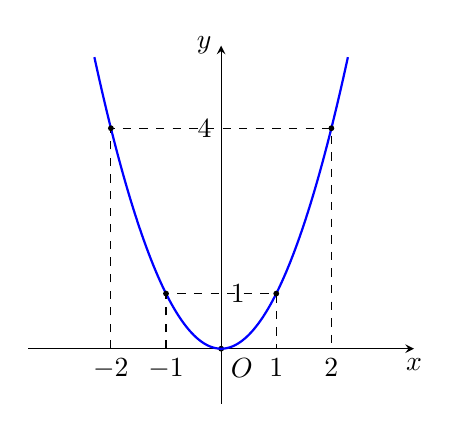
\begin{tikzpicture}[>=stealth, scale=0.7]
					\draw[->] (-3.5,0) -- (3.5,0) node[below] {$x$};
					\draw[->] (0,-1) -- (0,5.5) node[left] {$y$};
					\fill (0,0) circle (1.5pt) node[below right] {$O$};
					\draw[smooth, samples=100, domain=-2.3:2.3, thick, color=blue] plot(\x, {(\x)^2});
					\draw[dashed] (-2,0) node[below] {$-2$} -- (-2,4) -- (0,4) node[left] {$4$} -- (2,4) -- (2,0) node[below] {$2$};
					\draw[dashed] (-1,0) node[below] {$-1$} -- (-1,1) -- (0,1) node[right] {$1$} -- (1,1) -- (1,0) node[below] {$1$};
					\fill (-2,4) circle (1.5pt) (2,4) circle (1.5pt) (-1,1) circle (1.5pt) (1,1) circle (1.5pt);
				\end{tikzpicture}
			\end{center}
			\item Điểm thuộc $(P)$ có tung độ bằng $12$ nên $y = 12$.
			
			Thay $y = 12$ vào phương trình parabol $(P)$, ta được:
			$$x^2 = 12 \iff x = \pm \sqrt{12} = \pm 2\sqrt{3}.$$
			Vậy có hai điểm thỏa mãn yêu cầu đề bài là $(2\sqrt{3}; 12)$ và $(-2\sqrt{3}; 12)$.
		\end{enumerate}
	}
\end{bt}

\begin{bt}%[9D6H20-2]
% nguon: Đề tham khảo Tuyển sinh 10 năm học 2026-2027 Sở GD&ĐT TP.HCM - Cụm 6 Đề 2, Bài 2
	Cho phương trình $x^2 - 3x - 10 = 0$ có hai nghiệm phân biệt $x_1, x_2$. Không giải phương trình, hãy tính giá trị của biểu thức:
	$$Q = \dfrac{x_1 + 1}{x_2} + \dfrac{x_2 + 1}{x_1}.$$
	\loigiai{
		Phương trình $x^2 - 3x - 10 = 0$ có $a = 1, b = -3, c = -10$.
		
		Vì $a \cdot c = 1 \cdot (-10) = -10 < 0$ nên phương trình luôn có hai nghiệm phân biệt $x_1, x_2$.
		
		Theo định lí Viète, ta có:
		$$\begin{cases} x_1 + x_2 = 3 \\ x_1 x_2 = -10. \end{cases}$$
		Ta có:
		$$x_1^2 + x_2^2 = (x_1 + x_2)^2 - 2x_1 x_2 = 3^2 - 2 \cdot (-10) = 9 + 20 = 29.$$
		Quy đồng mẫu số biểu thức $Q$, ta được:
		$$Q = \dfrac{x_1(x_1 + 1) + x_2(x_2 + 1)}{x_1 x_2} = \dfrac{(x_1^2 + x_2^2) + (x_1 + x_2)}{x_1 x_2}.$$
		Thay số vào, ta được:
		$$Q = \dfrac{29 + 3}{-10} = \dfrac{32}{-10} = -\dfrac{16}{5} = -3{,}2.$$
		Vậy $Q = -\dfrac{16}{5}$.
	}
\end{bt}

\begin{bt}%[9D8H26-3]
% nguon: Đề tham khảo Tuyển sinh 10 năm học 2026-2027 Sở GD&ĐT TP.HCM - Cụm 6 Đề 2, Bài 3
	\begin{enumerate}[a)]
		\item Bạn Nam khảo sát môn học yêu thích nhất của $40$ bạn học sinh trong lớp và ghi lại kết quả: có $11$ bạn thích Toán, $8$ bạn thích Ngữ văn, $9$ bạn thích Lịch sử và $12$ bạn thích Thể dục. Xác định tần số và tần số tương đối của môn Lịch sử.
		\item Một hộp chứa $20$ tấm thẻ giống nhau được đánh số từ $1$ đến $20$. Rút ngẫu nhiên một tấm thẻ từ hộp. Tính xác suất của biến cố $A$: ``Số ghi trên tấm thẻ được rút ra lớn hơn $15$''.
	\end{enumerate}
	\loigiai{
		\begin{enumerate}[a)]
			\item Môn Lịch sử có $9$ bạn yêu thích nhất.
			
			Vậy tần số của môn Lịch sử là $9$.
			
			Tần số tương đối của môn Lịch sử là:
			$$f = \dfrac{9}{40} \cdot 100\% = 22{,}5\%.$$
			\item Số kết quả có thể xảy ra khi rút một tấm thẻ là $n(\Omega) = 20$.
			
			Các tấm thẻ có số ghi lớn hơn $15$ là các thẻ mang số: $16, 17, 18, 19, 20$.
			
			Do đó số kết quả thuận lợi cho biến cố $A$ là $n(A) = 5$.
			
			Xác suất của biến cố $A$ là:
			$$P(A) = \dfrac{n(A)}{n(\Omega)} = \dfrac{5}{20} = \dfrac{1}{4} = 0{,}25.$$
		\end{enumerate}
	}
\end{bt}

\begin{bt}%[9D6V21-3]
% nguon: Đề tham khảo Tuyển sinh 10 năm học 2026-2027 Sở GD&ĐT TP.HCM - Cụm 6 Đề 2, Bài 4
	Một khu đất hình chữ nhật có chiều dài là $1{,}57x + 10\text{ (m)}$. Người ta thiết kế một bồn hoa hình tròn bán kính $x\text{ (m)}$ tiếp xúc với hai cạnh kề của khu đất. Khoảng cách từ mép bồn hoa đến cạnh chiều dài đối diện là $2\text{ m}$, do đó chiều rộng của khu đất là $2x + 2\text{ (m)}$ (với $x > 0$).
	\begin{enumerate}[a)]
		\item Viết biểu thức theo $x$ tính diện tích phần đất còn lại sau khi đã làm bồn hoa.
		\item Biết diện tích phần đất còn lại là $54{,}71\text{ m}^2$, hãy tìm bán kính $x$ của bồn hoa. Lấy $\pi \approx 3{,}14$.
	\end{enumerate}
	\loigiai{
		\begin{enumerate}[a)]
			\item Diện tích của toàn bộ khu đất hình chữ nhật là:
			$$S_{\text{khu đất}} = (1{,}57x + 10)(2x + 2) = 3{,}14x^2 + 3{,}14x + 20x + 20 = 3{,}14x^2 + 23{,}14x + 20\text{ (m}^2).$$
			Diện tích của bồn hoa hình tròn bán kính $x$ là:
			$$S_{\text{hoa}} = \pi x^2 \approx 3{,}14x^2\text{ (m}^2).$$
			Diện tích phần đất còn lại sau khi làm bồn hoa là:
			$$S = S_{\text{khu đất}} - S_{\text{hoa}} = (3{,}14x^2 + 23{,}14x + 20) - 3{,}14x^2 = 23{,}14x + 20\text{ (m}^2).$$
			\item Theo giả thiết, diện tích phần đất còn lại là $54{,}71\text{ m}^2$ nên ta có phương trình:
			$$23{,}14x + 20 = 54{,}71 \iff 23{,}14x = 34{,}71 \iff x = \dfrac{34{,}71}{23{,}14} = 1{,}5\text{ (m) (thỏa mãn } x > 0).$$
			Vậy bán kính của bồn hoa là $x = 1{,}5\text{ m}$.
		\end{enumerate}
	}
\end{bt}

\begin{bt}%[9H0V31-3]
% nguon: Đề tham khảo Tuyển sinh 10 năm học 2026-2027 Sở GD&ĐT TP.HCM - Cụm 6 Đề 2, Bài 5
	Một hộp chứa đồ chơi dạng hình trụ kín hai đáy chứa vừa khít hai quả bóng hình cầu bằng nhau, có cùng bán kính $R$. Biết rằng hai quả bóng tiếp xúc với nhau, đồng thời tiếp xúc với hai đáy và xung quanh của hình trụ.
	\begin{enumerate}[a)]
		\item Hãy biểu diễn chiều cao $h$ và bán kính đáy $r$ của hình trụ theo bán kính $R$ của quả bóng.
		\item Biết thể tích của khối trụ là $120\text{ cm}^3$, hãy tính tổng thể tích của hai quả bóng hình cầu bên trong.
	\end{enumerate}
	\loigiai{
		\begin{enumerate}[a)]
			\item Vì hai quả bóng hình cầu bán kính $R$ xếp vừa khít trong hộp hình trụ và tiếp xúc nhau nên:
			
			Chiều cao của hình trụ bằng tổng hai đường kính của hai quả bóng:
			$$h = 2R + 2R = 4R.$$
			
			Bán kính đáy của hình trụ bằng bán kính của mỗi quả bóng:
			$$r = R.$$
			\item Thể tích của khối trụ được tính theo công thức:
			$$V_{\text{trụ}} = \pi r^2 h = \pi \cdot R^2 \cdot 4R = 4\pi R^3.$$
			Theo đề bài ta có $V_{\text{trụ}} = 120\text{ cm}^3$, suy ra:
			$$4\pi R^3 = 120 \iff \pi R^3 = 30\text{ (cm}^3).$$
			Thể tích của một quả bóng hình cầu là:
			$$V_{\text{cầu}} = \dfrac{4}{3}\pi R^3.$$
			Tổng thể tích của cả hai quả bóng hình cầu bên trong hộp là:
			$$V_{\text{tổng}} = 2 \cdot V_{\text{cầu}} = 2 \cdot \left(\dfrac{4}{3}\pi R^3\right) = \dfrac{8}{3}\pi R^3.$$
			Thay $\pi R^3 = 30\text{ cm}^3$ vào, ta được:
			$$V_{\text{tổng}} = \dfrac{8}{3} \cdot 30 = 80\text{ (cm}^3).$$
			Vậy tổng thể tích của hai quả bóng hình cầu là $80\text{ cm}^3$.
		\end{enumerate}
	}
\end{bt}

\begin{bt}%[9D1H3-4]
% nguon: Đề tham khảo Tuyển sinh 10 năm học 2026-2027 Sở GD&ĐT TP.HCM - Cụm 6 Đề 2, Bài 6
	Một hộ gia đình vay ngân hàng số tiền $100$ triệu đồng để sản xuất kinh doanh theo hình thức tính lãi kép kỳ hạn $1$ năm (nghĩa là sau mỗi năm, tiền lãi của năm đó được cộng dồn vào tiền vốn để tính lãi cho năm tiếp theo). Sau $2$ năm, hộ gia đình đó phải trả cho ngân hàng tổng cộng cả vốn lẫn lãi là $118\,810\,000$ đồng. Hỏi lãi suất cho vay hàng năm của ngân hàng là bao nhiêu phần trăm?
	\loigiai{
		Gọi $x$ (phần trăm) là lãi suất cho vay hàng năm của ngân hàng ($x > 0$).
		
		Số tiền cả vốn lẫn lãi sau năm thứ nhất là:
		$$100\,000\,000 \cdot \left(1 + \dfrac{x}{100}\right)\text{ (đồng)}.$$
		Số tiền cả vốn lẫn lãi sau năm thứ hai là:
		$$100\,000\,000 \cdot \left(1 + \dfrac{x}{100}\right)^2\text{ (đồng)}.$$
		Theo đề bài, sau $2$ năm tổng số tiền phải trả là $118\,810\,000$ đồng nên ta có phương trình:
		$$100\,000\,000 \cdot \left(1 + \dfrac{x}{100}\right)^2 = 118\,810\,000.$$
		Chia cả hai vế cho $100\,000\,000$, ta được:
		$$\left(1 + \dfrac{x}{100}\right)^2 = \dfrac{118\,810\,000}{100\,000\,000} = 1{,}1881.$$
		Vì $x > 0$ nên $1 + \dfrac{x}{100} > 0$, do đó:
		$$1 + \dfrac{x}{100} = \sqrt{1{,}1881} = 1{,}09 \iff \dfrac{x}{100} = 0{,}09 \iff x = 9.$$
		Vậy lãi suất cho vay hàng năm của ngân hàng là $9\%$/năm.
	}
\end{bt}

\begin{bt}%[9H9C29-3]
% nguon: Đề tham khảo Tuyển sinh 10 năm học 2026-2027 Sở GD&ĐT TP.HCM - Cụm 6 Đề 2, Bài 7
	Từ điểm $M$ nằm bên ngoài đường tròn $(O; R)$, kẻ hai tiếp tuyến $MP, MQ$ với đường tròn ($P, Q$ là hai tiếp điểm). Kẻ cát tuyến $MAB$ không đi qua tâm $O$ sao cho $A$ nằm giữa $M$ và $B$. Gọi $I$ là trung điểm của dây cung $AB$. Đoạn thẳng $PQ$ cắt đoạn thẳng $AB$ tại điểm $E$.
	\begin{enumerate}[a)]
		\item Chứng minh bốn điểm $M, P, O, Q$ cùng thuộc một đường tròn và $OM \perp PQ$.
		\item Chứng minh $MP^2 = MI \cdot ME$.
		\item Giả sử $PB = a$ và $A$ là trung điểm của đoạn thẳng $MB$. Tính độ dài đoạn thẳng $PA$ theo $a$.
	\end{enumerate}
	\loigiai{
		\begin{center}
			\begin{tikzpicture}[>=stealth, scale=0.9]
				\coordinate (O) at (0,0);
				\def\r{2.2}
				\draw (O) circle (\r);
				\coordinate (M) at (-5,0);
				\pgfmathsetmacro{\distM}{5}
				\pgfmathsetmacro{\alphaM}{acos(\r/\distM)}
				\coordinate (P) at ({\alphaM}:\r);
				\coordinate (Q) at ({-\alphaM}:\r);
				\draw (M) -- (P) node[above] {$P$};
				\draw (M) -- (Q) node[below] {$Q$};
				\draw (O) -- (P);
				\draw (O) -- (Q);
				\draw (O) -- (M);
				\draw (P) -- (Q);
				\coordinate (A) at (-2.5, 1.25);
				\path (M) -- (A) coordinate[pos=2] (B);
				\draw (M) -- (B);
				\coordinate (I) at ($(A)!0.5!(B)$);
				\coordinate (E) at (intersection of P--Q and M--B);
				\draw (P) -- (A) node[above left] {$A$};
				\draw (P) -- (B) node[right] {$B$};
				\draw (O) -- (I);
				\node at (O) [below right] {$O$};
				\node at (M) [left] {$M$};
				\node at (I) [above] {$I$};
				\node at (E) [below left] {$E$};
				\fill (O) circle (1.5pt) (M) circle (1.5pt) (P) circle (1.5pt) (Q) circle (1.5pt) (A) circle (1.5pt) (B) circle (1.5pt) (I) circle (1.5pt) (E) circle (1.5pt);
			\end{tikzpicture}
		\end{center}
		\begin{enumerate}[a)]
			\item Vì $MP, MQ$ là hai tiếp tuyến của $(O)$ nên $\widehat{MPO} = 90^\circ$ và $\widehat{MQO} = 90^\circ$.
			
			Xét tứ giác $MPOQ$ có $\widehat{MPO} + \widehat{MQO} = 90^\circ + 90^\circ = 180^\circ$, do đó $MPOQ$ là tứ giác nội tiếp đường tròn đường kính $MO$.
			
			Lại có $MP = MQ$ (tính chất hai tiếp tuyến cắt nhau) và $OP = OQ = R$ nên $OM$ là đường trung trực của đoạn thẳng $PQ$.
			
			Suy ra $OM \perp PQ$.
			\item Gọi $H$ là giao điểm của $OM$ và $PQ$. Trong tam giác vuông $MPO$ có đường cao $PH$, ta có hệ thức lượng:
			$$MP^2 = MH \cdot MO.$$
			Vì $I$ là trung điểm của dây cung $AB$ nên $OI \perp AB \implies \widehat{MIO} = 90^\circ$.
			
			Xét tứ giác $OIEH$ có $\widehat{MIO} = 90^\circ$ và $\widehat{MHE} = 90^\circ$.
			
			Do đó $\Delta MHE \backsim \Delta MIO\text{ (g-g)}$ (vì có $\widehat{OMI}$ chung và $\widehat{MHE} = \widehat{MIO} = 90^\circ$).
			
			Suy ra:
			$$\dfrac{MH}{MI} = \dfrac{ME}{MO} \implies MH \cdot MO = MI \cdot ME.$$
			Từ đó suy ra $MP^2 = MI \cdot ME$.
			\item Xét $\Delta MPA$ và $\Delta MBP$ có:
			$$\widehat{PMB}\text{ chung};$$
			$\widehat{MPA} = \widehat{MBP}$ (góc tạo bởi tia tiếp tuyến và dây cung và góc nội tiếp cùng chắn cung $AP$).
			
			Do đó $\Delta MPA \backsim \Delta MBP\text{ (g-g)}$.
			
			Suy ra:
			$$\dfrac{MP}{MB} = \dfrac{MA}{MP} = \dfrac{PA}{PB} \implies MP^2 = MA \cdot MB.$$
			Theo giả thiết, $A$ là trung điểm của đoạn thẳng $MB$ nên $MB = 2MA$.
			
			Thay vào hệ thức trên, ta được:
			$$MP^2 = MA \cdot (2MA) = 2MA^2 \implies MP = MA\sqrt{2}.$$
			Từ tỉ số đồng dạng $\dfrac{MA}{MP} = \dfrac{PA}{PB}$, ta có:
			$$PA = PB \cdot \dfrac{MA}{MP} = a \cdot \dfrac{MA}{MA\sqrt{2}} = \dfrac{a}{\sqrt{2}} = \dfrac{a\sqrt{2}}{2}.$$
			Vậy $PA = \dfrac{a\sqrt{2}}{2}$.
		\end{enumerate}
	}
\end{bt}
